 \documentclass{article}
\usepackage[utf8]{inputenc}
\usepackage[a4paper, total={7in, 10in}]{geometry}
\usepackage{braket}
\usepackage{xcolor}
\usepackage{amsmath}
\usepackage{amssymb}
\usepackage{amsfonts}
\usepackage{graphicx}
\usepackage{svg}
\usepackage{float}
\usepackage{tikz}
\usepackage[ruled,vlined]{algorithm2e}
\usepackage{multicol}
\usepackage[backend=biber,style=alphabetic,sorting=ynt]{biblatex}
\usepackage{xcolor}
%\addbibresource{sample.bib} %Import the bibliography file

\newcommand{\commentt}[1]{\textcolor{blue}{ \textbf{[COMMENT]} #1}}
\newcommand{\ctt}[1]{\commentt{#1}}
\newcommand{\prb}[1]{ \mathbf{Pr} \left[ {#1} \right]}
\newcommand{\onotation}[1]{\(\mathcal{O} \left( {#1}  \right) \)}
\newcommand{\ona}[1]{\onotation{#1}}
\newcommand{\PSI}{{\ket{\psi}}}
\newcommand{\LESn}{\ket{\psi_n}}
\newcommand{\LESa}{\ket{\phi_n}}
\newcommand{\LESs}{\frac{1}{\sqrt{n}}\sum_{i}{\ket{\left(0^{i}10^{n-i}\right)^{n}}}}
\newcommand{\Hn}{\mathcal{H}_{n}}
\newcommand{\Ep}{\frac{1}{\sqrt{2^n}}\sum^{2^n}_{x}{ \ket{xx}}}
\newcommand{\HON}{\ket{\psi_{\text{honest}}}}
\newcommand{\Lemma}{\paragraph{Lemma.}}


\setlength{\columnsep}{0.6cm}

\newcommand{\Gz}{ G_{z}^{\delta} } 

\begin{document}

\title{Quantum LTC With Positive Rate}
\author{David Ponarovsky}
\maketitle
\begin{multicols*}{2}
\newcommand{ \Hw }{ \delta\Delta -\Delta^{\frac{1}{2}-\varepsilon}/\delta  }
	\newcommand{ \Nw }{ \Delta^{\frac{3}{2}-\varepsilon}} 
	  \newcommand{ \Gu } { \Gamma^{\cup} }
	  \newcommand{ \Guq } { \Gamma^{\cup, \square} }

    	\newcommand{ \Gsa } {\Gamma_{\square_{1}} }
	\newcommand{ \Gsb } {\Gamma_{\square_{2}} }
        \newcommand{ \Aa } { C_{A_{1}}}  
	\newcommand{ \Ab } { C_{A_{2}}}
	\newcommand{ \Ac } { C_{A_{3}}}
	\newcommand{ \Aab } { \Aa \otimes \Ab } 
	\newcommand{ \Aac } { \Aa \otimes \Ac }
	\newcommand{ \Aabc } { \Aa \otimes \Ab \otimes \Ac }
	\newcommand{ \Aabp } { \Aa^{\perp} \otimes \Ab^{\perp} } 
	\newcommand{ \Aacp } { \Aa^{\perp} \otimes \Ac^{\perp} }
	\newcommand{ \Aabcp } { \Aa^{\perp} \otimes \Ab^{\perp} \otimes \Ac^{\perp} }
	\newcommand{ \Aabpp } { \left( \Aabp \right)^\perp } 
	\newcommand{ \Aacpp } { \left( \Aacp \right)^\perp }
	\newcommand{ \Aabcpp } { \left( \Aabcp \right)^\perp }
	\newcommand{ \YY } {  y_{1}y_{2}^{\top} }
	\newcommand{ \ZZ } {  z_{1}z_{2}^{\top} } 
	\newcommand{ \TT } { \tilde{\tau} } 


  \paragraph{preamble.} preamble.  
  \begin{figure}[H]
            %\label{fig:square}
            \begin{center}
            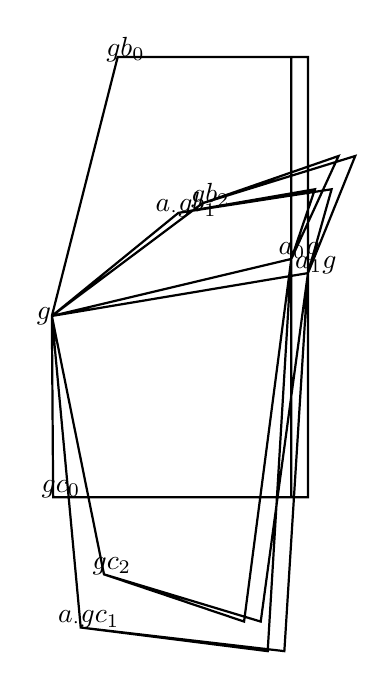
\begin{tikzpicture}
            \draw[thick](0,0)(0,0) -- (0.8356986771932391,3.28807199939629) -- (3.040791378018191,3.28807199939629) -- (3.040791378018191,0.7242747901375232) -- (0,0)
(0,0) -- (1.6065628374588468,1.3092172254653247) -- (3.340791378018191,1.6092172254653248) -- (3.040791378018191,0.7242747901375232) -- (0,0)
(0,0) -- (1.9124016102802752,1.4316328111562795) -- (3.640791378018191,2.0316328111562796) -- (3.040791378018191,0.7242747901375232) -- (0,0)
(0,0) -- (0.8356986771932391,3.28807199939629) -- (3.2524768628504996,3.28807199939629) -- (3.2524768628504996,0.5446525128752887) -- (0,0)
(0,0) -- (1.6065628374588468,1.3092172254653247) -- (3.5524768628504995,1.6092172254653248) -- (3.2524768628504996,0.5446525128752887) -- (0,0)
(0,0) -- (1.9124016102802752,1.4316328111562795) -- (3.8524768628504997,2.0316328111562796) -- (3.2524768628504996,0.5446525128752887) -- (0,0)
(0,0) -- (0.01633002920865656,-2.301221660209101) -- (3.040791378018191,-2.301221660209101) -- (3.040791378018191,0.7242747901375232) -- (0,0)
(0,0) -- (0.36634654014574397,-3.956522669779943) -- (2.740791378018191,-4.256522669779943) -- (3.040791378018191,0.7242747901375232) -- (0,0)
(0,0) -- (0.6620178371008967,-3.28113652238806) -- (2.440791378018191,-3.88113652238806) -- (3.040791378018191,0.7242747901375232) -- (0,0)
(0,0) -- (0.01633002920865656,-2.301221660209101) -- (3.2524768628504996,-2.301221660209101) -- (3.2524768628504996,0.5446525128752887) -- (0,0)
(0,0) -- (0.36634654014574397,-3.956522669779943) -- (2.9524768628505,-4.256522669779943) -- (3.2524768628504996,0.5446525128752887) -- (0,0)
(0,0) -- (0.6620178371008967,-3.28113652238806) -- (2.6524768628504996,-3.88113652238806) -- (3.2524768628504996,0.5446525128752887) -- (0,0)
;
\node at (-0.1,0) {$ g $};
\node at (3.140791378018191,0.8242747901375231) {$ a_{ 0 }g $};
\node at (3.3524768628504997,0.6446525128752887) {$ a_{ 1 }g $};
\node at (0.9356986771932391,3.3880719993962902) {$ gb_{ 0 } $};
\node at (1.7065628374588468,1.4092172254653248) {$ a_{\cdot} gb_{ 1 } $};
\node at (2.0124016102802753,1.5316328111562796) {$ gb_{ 2 } $};
\node at (0.11633002920865657,-2.201221660209101) {$ gc_{ 0 } $};
\node at (0.46634654014574395,-3.856522669779943) {$ a_{\cdot} gc_{ 1 } $};
\node at (0.7620178371008967,-3.18113652238806) {$ gc_{ 2 } $};

            \end{tikzpicture}
            \end{center}
            \caption{Square of the complex, with edges $(g,ag), (agb, gb) \in E_A,
            (g,gb), (agb, ag) \in E_B.$ \label{fig:square}
            }
            \end{figure}
 \begin{figure}[H]
            %\label{fig:square}
            \begin{center}
            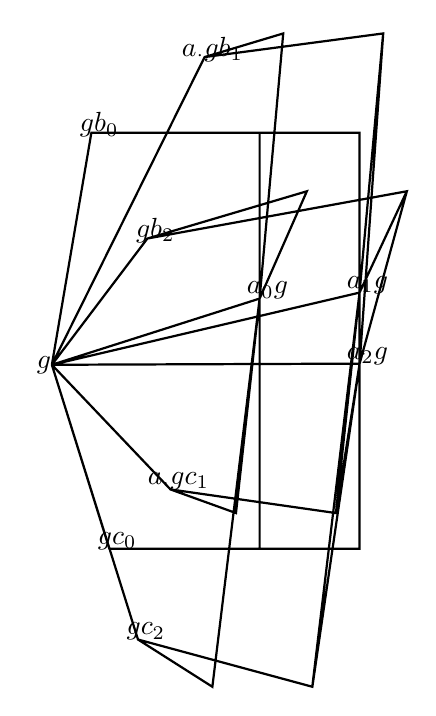
\begin{tikzpicture}
            \draw[thick](0,0)(0,0) -- (0.501503179285874,2.9455924878285975) -- (2.6383109450326048,2.9455924878285975) -- (2.6383109450326048,0.8408208908375948) -- (0,0)
(0,0) -- (1.9397936917973473,3.9078783590571287) -- (2.9383109450326046,4.207878359057129) -- (2.6383109450326048,0.8408208908375948) -- (0,0)
(0,0) -- (1.2132869661124364,1.6035259070958463) -- (3.238310945032605,2.2035259070958464) -- (2.6383109450326048,0.8408208908375948) -- (0,0)
(0,0) -- (0.501503179285874,2.9455924878285975) -- (3.907223367619018,2.9455924878285975) -- (3.907223367619018,0.9165189300547416) -- (0,0)
(0,0) -- (1.9397936917973473,3.9078783590571287) -- (4.207223367619018,4.207878359057129) -- (3.907223367619018,0.9165189300547416) -- (0,0)
(0,0) -- (1.2132869661124364,1.6035259070958463) -- (4.507223367619018,2.2035259070958464) -- (3.907223367619018,0.9165189300547416) -- (0,0)
(0,0) -- (0.501503179285874,2.9455924878285975) -- (3.908229241905875,2.9455924878285975) -- (3.908229241905875,0.01444114542328423) -- (0,0)
(0,0) -- (1.9397936917973473,3.9078783590571287) -- (4.208229241905875,4.207878359057129) -- (3.908229241905875,0.01444114542328423) -- (0,0)
(0,0) -- (1.2132869661124364,1.6035259070958463) -- (4.508229241905875,2.2035259070958464) -- (3.908229241905875,0.01444114542328423) -- (0,0)
(0,0) -- (0.7301612987022605,-2.3364410355972645) -- (2.6383109450326048,-2.3364410355972645) -- (2.6383109450326048,0.8408208908375948) -- (0,0)
(0,0) -- (1.506221923477486,-1.5830799221994336) -- (2.338310945032605,-1.8830799221994337) -- (2.6383109450326048,0.8408208908375948) -- (0,0)
(0,0) -- (1.0937649628058874,-3.4892300395197187) -- (2.0383109450326047,-4.089230039519719) -- (2.6383109450326048,0.8408208908375948) -- (0,0)
(0,0) -- (0.7301612987022605,-2.3364410355972645) -- (3.907223367619018,-2.3364410355972645) -- (3.907223367619018,0.9165189300547416) -- (0,0)
(0,0) -- (1.506221923477486,-1.5830799221994336) -- (3.607223367619018,-1.8830799221994337) -- (3.907223367619018,0.9165189300547416) -- (0,0)
(0,0) -- (1.0937649628058874,-3.4892300395197187) -- (3.307223367619018,-4.089230039519719) -- (3.907223367619018,0.9165189300547416) -- (0,0)
(0,0) -- (0.7301612987022605,-2.3364410355972645) -- (3.908229241905875,-2.3364410355972645) -- (3.908229241905875,0.01444114542328423) -- (0,0)
(0,0) -- (1.506221923477486,-1.5830799221994336) -- (3.608229241905875,-1.8830799221994337) -- (3.908229241905875,0.01444114542328423) -- (0,0)
(0,0) -- (1.0937649628058874,-3.4892300395197187) -- (3.3082292419058748,-4.089230039519719) -- (3.908229241905875,0.01444114542328423) -- (0,0)
;
\node at (-0.1,0) {$ g $};
\node at (2.738310945032605,0.9408208908375948) {$ a_{ 0 }g $};
\node at (4.007223367619018,1.0165189300547417) {$ a_{ 1 }g $};
\node at (4.008229241905875,0.11444114542328424) {$ a_{ 2 }g $};
\node at (0.6015031792858739,3.0455924878285976) {$ gb_{ 0 } $};
\node at (2.0397936917973474,4.007878359057129) {$ a_{\cdot} gb_{ 1 } $};
\node at (1.3132869661124364,1.7035259070958464) {$ gb_{ 2 } $};
\node at (0.8301612987022605,-2.2364410355972644) {$ gc_{ 0 } $};
\node at (1.6062219234774862,-1.4830799221994335) {$ a_{\cdot} gc_{ 1 } $};
\node at (1.1937649628058875,-3.3892300395197186) {$ gc_{ 2 } $};

            \end{tikzpicture}
            \end{center}
            \caption{Square of the complex, with edges $(g,ag), (agb, gb) \in E_A,
            (g,gb), (agb, ag) \in E_B.$ \label{fig:square}
            }
            \end{figure}
 \begin{figure}[H]
            %\label{fig:square}
            \begin{center}
            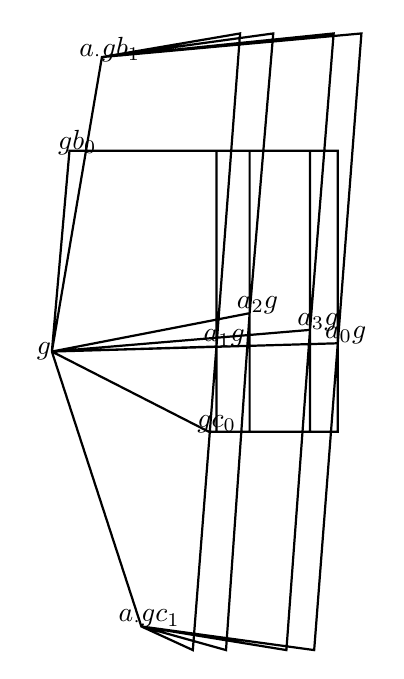
\begin{tikzpicture}
            \draw[thick](0,0)(0,0) -- (0.22349021222858734,2.549634566662319) -- (3.631198357448021,2.549634566662319) -- (3.631198357448021,0.10508357689661038) -- (0,0)
(0,0) -- (0.6355659756822423,3.7399727475863305) -- (3.9311983574480207,4.03997274758633) -- (3.631198357448021,0.10508357689661038) -- (0,0)
(0,0) -- (0.22349021222858734,2.549634566662319) -- (2.090133649138273,2.549634566662319) -- (2.090133649138273,0.06364077812186127) -- (0,0)
(0,0) -- (0.6355659756822423,3.7399727475863305) -- (2.390133649138273,4.03997274758633) -- (2.090133649138273,0.06364077812186127) -- (0,0)
(0,0) -- (0.22349021222858734,2.549634566662319) -- (2.5115530227717526,2.549634566662319) -- (2.5115530227717526,0.4871771240447366) -- (0,0)
(0,0) -- (0.6355659756822423,3.7399727475863305) -- (2.8115530227717525,4.03997274758633) -- (2.5115530227717526,0.4871771240447366) -- (0,0)
(0,0) -- (0.22349021222858734,2.549634566662319) -- (3.2785232058564686,2.549634566662319) -- (3.2785232058564686,0.275282854541672) -- (0,0)
(0,0) -- (0.6355659756822423,3.7399727475863305) -- (3.5785232058564684,4.03997274758633) -- (3.2785232058564686,0.275282854541672) -- (0,0)
(0,0) -- (1.9933476287778278,-1.0185411018554078) -- (3.631198357448021,-1.0185411018554078) -- (3.631198357448021,0.10508357689661038) -- (0,0)
(0,0) -- (1.1365663502008316,-3.491249195019196) -- (3.331198357448021,-3.791249195019196) -- (3.631198357448021,0.10508357689661038) -- (0,0)
(0,0) -- (1.9933476287778278,-1.0185411018554078) -- (2.090133649138273,-1.0185411018554078) -- (2.090133649138273,0.06364077812186127) -- (0,0)
(0,0) -- (1.1365663502008316,-3.491249195019196) -- (1.790133649138273,-3.791249195019196) -- (2.090133649138273,0.06364077812186127) -- (0,0)
(0,0) -- (1.9933476287778278,-1.0185411018554078) -- (2.5115530227717526,-1.0185411018554078) -- (2.5115530227717526,0.4871771240447366) -- (0,0)
(0,0) -- (1.1365663502008316,-3.491249195019196) -- (2.211553022771753,-3.791249195019196) -- (2.5115530227717526,0.4871771240447366) -- (0,0)
(0,0) -- (1.9933476287778278,-1.0185411018554078) -- (3.2785232058564686,-1.0185411018554078) -- (3.2785232058564686,0.275282854541672) -- (0,0)
(0,0) -- (1.1365663502008316,-3.491249195019196) -- (2.978523205856469,-3.791249195019196) -- (3.2785232058564686,0.275282854541672) -- (0,0)
;
\node at (-0.1,0) {$ g $};
\node at (3.731198357448021,0.2050835768966104) {$ a_{ 0 }g $};
\node at (2.1901336491382732,0.16364077812186129) {$ a_{ 1 }g $};
\node at (2.6115530227717527,0.5871771240447367) {$ a_{ 2 }g $};
\node at (3.3785232058564687,0.375282854541672) {$ a_{ 3 }g $};
\node at (0.3234902122285873,2.649634566662319) {$ gb_{ 0 } $};
\node at (0.7355659756822422,3.8399727475863306) {$ a_{\cdot} gb_{ 1 } $};
\node at (2.0933476287778277,-0.9185411018554078) {$ gc_{ 0 } $};
\node at (1.2365663502008317,-3.391249195019196) {$ a_{\cdot} gc_{ 1 } $};

            \end{tikzpicture}
            \end{center}
            \caption{Square of the complex, with edges $(g,ag), (agb, gb) \in E_A,
            (g,gb), (agb, ag) \in E_B.$ \label{fig:square}
            }
            \end{figure}
 \begin{figure}[H]
            %\label{fig:square}
            \begin{center}
            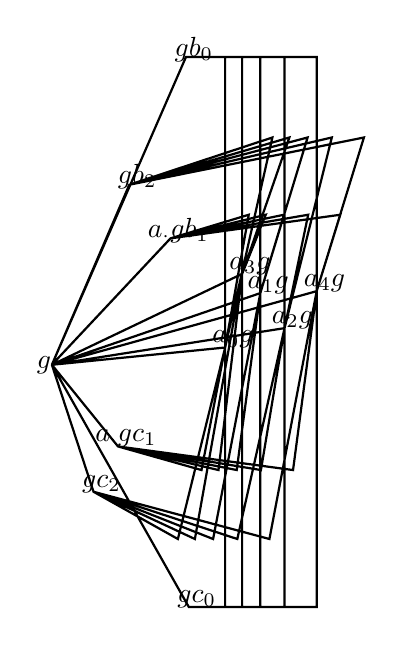
\begin{tikzpicture}
            \draw[thick](0,0)(0,0) -- (1.7026864139869315,3.907790727190659) -- (2.200409644953861,3.907790727190659) -- (2.200409644953861,0.21911409474615354) -- (0,0)
(0,0) -- (1.506612509743652,1.6052981307336436) -- (2.500409644953861,1.9052981307336436) -- (2.200409644953861,0.21911409474615354) -- (0,0)
(0,0) -- (0.9835240497069608,2.2864570346746342) -- (2.800409644953861,2.8864570346746343) -- (2.200409644953861,0.21911409474615354) -- (0,0)
(0,0) -- (1.7026864139869315,3.907790727190659) -- (2.647546147048131,3.907790727190659) -- (2.647546147048131,0.9103667243774517) -- (0,0)
(0,0) -- (1.506612509743652,1.6052981307336436) -- (2.947546147048131,1.9052981307336436) -- (2.647546147048131,0.9103667243774517) -- (0,0)
(0,0) -- (0.9835240497069608,2.2864570346746342) -- (3.2475461470481313,2.8864570346746343) -- (2.647546147048131,0.9103667243774517) -- (0,0)
(0,0) -- (1.7026864139869315,3.907790727190659) -- (2.9551179432814214,3.907790727190659) -- (2.9551179432814214,0.4652245373835369) -- (0,0)
(0,0) -- (1.506612509743652,1.6052981307336436) -- (3.2551179432814212,1.9052981307336436) -- (2.9551179432814214,0.4652245373835369) -- (0,0)
(0,0) -- (0.9835240497069608,2.2864570346746342) -- (3.5551179432814215,2.8864570346746343) -- (2.9551179432814214,0.4652245373835369) -- (0,0)
(0,0) -- (1.7026864139869315,3.907790727190659) -- (2.416274001051143,3.907790727190659) -- (2.416274001051143,1.1544902801264993) -- (0,0)
(0,0) -- (1.506612509743652,1.6052981307336436) -- (2.716274001051143,1.9052981307336436) -- (2.416274001051143,1.1544902801264993) -- (0,0)
(0,0) -- (0.9835240497069608,2.2864570346746342) -- (3.0162740010511433,2.8864570346746343) -- (2.416274001051143,1.1544902801264993) -- (0,0)
(0,0) -- (1.7026864139869315,3.907790727190659) -- (3.3629151396003767,3.907790727190659) -- (3.3629151396003767,0.9349120550514649) -- (0,0)
(0,0) -- (1.506612509743652,1.6052981307336436) -- (3.6629151396003765,1.9052981307336436) -- (3.3629151396003767,0.9349120550514649) -- (0,0)
(0,0) -- (0.9835240497069608,2.2864570346746342) -- (3.962915139600377,2.8864570346746343) -- (3.3629151396003767,0.9349120550514649) -- (0,0)
(0,0) -- (1.7399337123206575,-3.0775865247483907) -- (2.200409644953861,-3.0775865247483907) -- (2.200409644953861,0.21911409474615354) -- (0,0)
(0,0) -- (0.839964748804038,-1.0370190538070716) -- (1.900409644953861,-1.3370190538070716) -- (2.200409644953861,0.21911409474615354) -- (0,0)
(0,0) -- (0.5289578275211979,-1.6127106785695093) -- (1.600409644953861,-2.2127106785695094) -- (2.200409644953861,0.21911409474615354) -- (0,0)
(0,0) -- (1.7399337123206575,-3.0775865247483907) -- (2.647546147048131,-3.0775865247483907) -- (2.647546147048131,0.9103667243774517) -- (0,0)
(0,0) -- (0.839964748804038,-1.0370190538070716) -- (2.3475461470481314,-1.3370190538070716) -- (2.647546147048131,0.9103667243774517) -- (0,0)
(0,0) -- (0.5289578275211979,-1.6127106785695093) -- (2.047546147048131,-2.2127106785695094) -- (2.647546147048131,0.9103667243774517) -- (0,0)
(0,0) -- (1.7399337123206575,-3.0775865247483907) -- (2.9551179432814214,-3.0775865247483907) -- (2.9551179432814214,0.4652245373835369) -- (0,0)
(0,0) -- (0.839964748804038,-1.0370190538070716) -- (2.6551179432814216,-1.3370190538070716) -- (2.9551179432814214,0.4652245373835369) -- (0,0)
(0,0) -- (0.5289578275211979,-1.6127106785695093) -- (2.3551179432814213,-2.2127106785695094) -- (2.9551179432814214,0.4652245373835369) -- (0,0)
(0,0) -- (1.7399337123206575,-3.0775865247483907) -- (2.416274001051143,-3.0775865247483907) -- (2.416274001051143,1.1544902801264993) -- (0,0)
(0,0) -- (0.839964748804038,-1.0370190538070716) -- (2.1162740010511434,-1.3370190538070716) -- (2.416274001051143,1.1544902801264993) -- (0,0)
(0,0) -- (0.5289578275211979,-1.6127106785695093) -- (1.8162740010511431,-2.2127106785695094) -- (2.416274001051143,1.1544902801264993) -- (0,0)
(0,0) -- (1.7399337123206575,-3.0775865247483907) -- (3.3629151396003767,-3.0775865247483907) -- (3.3629151396003767,0.9349120550514649) -- (0,0)
(0,0) -- (0.839964748804038,-1.0370190538070716) -- (3.062915139600377,-1.3370190538070716) -- (3.3629151396003767,0.9349120550514649) -- (0,0)
(0,0) -- (0.5289578275211979,-1.6127106785695093) -- (2.7629151396003766,-2.2127106785695094) -- (3.3629151396003767,0.9349120550514649) -- (0,0)
;
\node at (-0.1,0) {$ g $};
\node at (2.300409644953861,0.31911409474615354) {$ a_{ 0 }g $};
\node at (2.7475461470481313,1.0103667243774517) {$ a_{ 1 }g $};
\node at (3.0551179432814215,0.565224537383537) {$ a_{ 2 }g $};
\node at (2.5162740010511433,1.2544902801264994) {$ a_{ 3 }g $};
\node at (3.462915139600377,1.034912055051465) {$ a_{ 4 }g $};
\node at (1.8026864139869316,4.007790727190659) {$ gb_{ 0 } $};
\node at (1.606612509743652,1.7052981307336437) {$ a_{\cdot} gb_{ 1 } $};
\node at (1.083524049706961,2.3864570346746343) {$ gb_{ 2 } $};
\node at (1.8399337123206576,-2.9775865247483906) {$ gc_{ 0 } $};
\node at (0.939964748804038,-0.9370190538070716) {$ a_{\cdot} gc_{ 1 } $};
\node at (0.6289578275211979,-1.5127106785695092) {$ gc_{ 2 } $};

            \end{tikzpicture}
            \end{center}
            \caption{Square of the complex, with edges $(g,ag), (agb, gb) \in E_A,
            (g,gb), (agb, ag) \in E_B.$ \label{fig:square}
            }
            \end{figure}
 \begin{figure}[H]
            %\label{fig:square}
            \begin{center}
            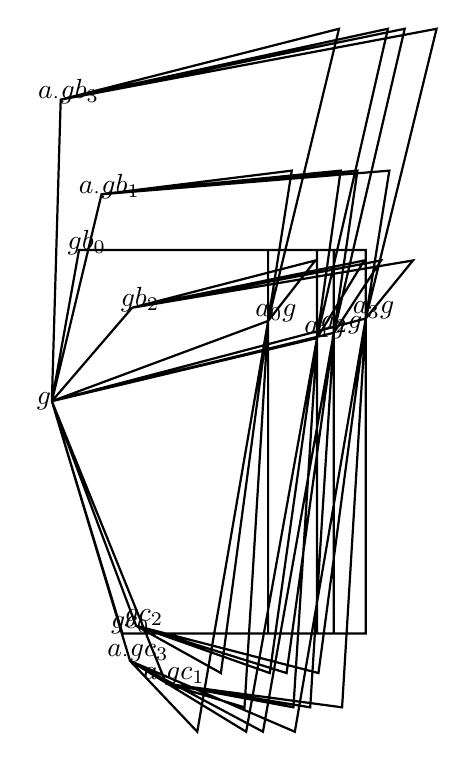
\begin{tikzpicture}
            \draw[thick](0,0)(0,0) -- (0.3447049673896341,1.9196300464435065) -- (2.7464840736150062,1.9196300464435065) -- (2.7464840736150062,1.0192982382153466) -- (0,0)
(0,0) -- (0.6306894992512635,2.627900053808133) -- (3.046484073615006,2.927900053808133) -- (2.7464840736150062,1.0192982382153466) -- (0,0)
(0,0) -- (1.0198555913606664,1.1871974527729874) -- (3.3464840736150063,1.7871974527729875) -- (2.7464840736150062,1.0192982382153466) -- (0,0)
(0,0) -- (0.11215982679887015,3.8295216604458107) -- (3.646484073615006,4.72952166044581) -- (2.7464840736150062,1.0192982382153466) -- (0,0)
(0,0) -- (0.3447049673896341,1.9196300464435065) -- (3.3674526560351072,1.9196300464435065) -- (3.3674526560351072,0.8015348543820469) -- (0,0)
(0,0) -- (0.6306894992512635,2.627900053808133) -- (3.667452656035107,2.927900053808133) -- (3.3674526560351072,0.8015348543820469) -- (0,0)
(0,0) -- (1.0198555913606664,1.1871974527729874) -- (3.9674526560351073,1.7871974527729875) -- (3.3674526560351072,0.8015348543820469) -- (0,0)
(0,0) -- (0.11215982679887015,3.8295216604458107) -- (4.267452656035108,4.72952166044581) -- (3.3674526560351072,0.8015348543820469) -- (0,0)
(0,0) -- (0.3447049673896341,1.9196300464435065) -- (3.5808911758699593,1.9196300464435065) -- (3.5808911758699593,0.8685791412196449) -- (0,0)
(0,0) -- (0.6306894992512635,2.627900053808133) -- (3.880891175869959,2.927900053808133) -- (3.5808911758699593,0.8685791412196449) -- (0,0)
(0,0) -- (1.0198555913606664,1.1871974527729874) -- (4.180891175869959,1.7871974527729875) -- (3.5808911758699593,0.8685791412196449) -- (0,0)
(0,0) -- (0.11215982679887015,3.8295216604458107) -- (4.480891175869959,4.72952166044581) -- (3.5808911758699593,0.8685791412196449) -- (0,0)
(0,0) -- (0.3447049673896341,1.9196300464435065) -- (3.9858095271852463,1.9196300464435065) -- (3.9858095271852463,1.0501964299440854) -- (0,0)
(0,0) -- (0.6306894992512635,2.627900053808133) -- (4.285809527185246,2.927900053808133) -- (3.9858095271852463,1.0501964299440854) -- (0,0)
(0,0) -- (1.0198555913606664,1.1871974527729874) -- (4.585809527185246,1.7871974527729875) -- (3.9858095271852463,1.0501964299440854) -- (0,0)
(0,0) -- (0.11215982679887015,3.8295216604458107) -- (4.885809527185247,4.72952166044581) -- (3.9858095271852463,1.0501964299440854) -- (0,0)
(0,0) -- (0.8965956298081361,-2.949317110598156) -- (2.7464840736150062,-2.949317110598156) -- (2.7464840736150062,1.0192982382153466) -- (0,0)
(0,0) -- (1.4526374503401271,-3.5880743210992385) -- (2.4464840736150064,-3.8880743210992383) -- (2.7464840736150062,1.0192982382153466) -- (0,0)
(0,0) -- (1.0704127445309062,-2.852816641270199) -- (2.146484073615006,-3.452816641270199) -- (2.7464840736150062,1.0192982382153466) -- (0,0)
(0,0) -- (0.9930629934694448,-3.2981044627860965) -- (1.8464840736150063,-4.198104462786096) -- (2.7464840736150062,1.0192982382153466) -- (0,0)
(0,0) -- (0.8965956298081361,-2.949317110598156) -- (3.3674526560351072,-2.949317110598156) -- (3.3674526560351072,0.8015348543820469) -- (0,0)
(0,0) -- (1.4526374503401271,-3.5880743210992385) -- (3.0674526560351074,-3.8880743210992383) -- (3.3674526560351072,0.8015348543820469) -- (0,0)
(0,0) -- (1.0704127445309062,-2.852816641270199) -- (2.767452656035107,-3.452816641270199) -- (3.3674526560351072,0.8015348543820469) -- (0,0)
(0,0) -- (0.9930629934694448,-3.2981044627860965) -- (2.4674526560351073,-4.198104462786096) -- (3.3674526560351072,0.8015348543820469) -- (0,0)
(0,0) -- (0.8965956298081361,-2.949317110598156) -- (3.5808911758699593,-2.949317110598156) -- (3.5808911758699593,0.8685791412196449) -- (0,0)
(0,0) -- (1.4526374503401271,-3.5880743210992385) -- (3.2808911758699595,-3.8880743210992383) -- (3.5808911758699593,0.8685791412196449) -- (0,0)
(0,0) -- (1.0704127445309062,-2.852816641270199) -- (2.980891175869959,-3.452816641270199) -- (3.5808911758699593,0.8685791412196449) -- (0,0)
(0,0) -- (0.9930629934694448,-3.2981044627860965) -- (2.6808911758699594,-4.198104462786096) -- (3.5808911758699593,0.8685791412196449) -- (0,0)
(0,0) -- (0.8965956298081361,-2.949317110598156) -- (3.9858095271852463,-2.949317110598156) -- (3.9858095271852463,1.0501964299440854) -- (0,0)
(0,0) -- (1.4526374503401271,-3.5880743210992385) -- (3.6858095271852465,-3.8880743210992383) -- (3.9858095271852463,1.0501964299440854) -- (0,0)
(0,0) -- (1.0704127445309062,-2.852816641270199) -- (3.385809527185246,-3.452816641270199) -- (3.9858095271852463,1.0501964299440854) -- (0,0)
(0,0) -- (0.9930629934694448,-3.2981044627860965) -- (3.0858095271852464,-4.198104462786096) -- (3.9858095271852463,1.0501964299440854) -- (0,0)
;
\node at (-0.1,0) {$ g $};
\node at (2.8464840736150063,1.1192982382153467) {$ a_{ 0 }g $};
\node at (3.4674526560351073,0.9015348543820468) {$ a_{ 1 }g $};
\node at (3.6808911758699594,0.9685791412196448) {$ a_{ 2 }g $};
\node at (4.085809527185246,1.1501964299440854) {$ a_{ 3 }g $};
\node at (0.44470496738963405,2.0196300464435066) {$ gb_{ 0 } $};
\node at (0.7306894992512635,2.727900053808133) {$ a_{\cdot} gb_{ 1 } $};
\node at (1.1198555913606665,1.2871974527729875) {$ gb_{ 2 } $};
\node at (0.21215982679887016,3.9295216604458107) {$ a_{\cdot} gb_{ 3 } $};
\node at (0.9965956298081361,-2.849317110598156) {$ gc_{ 0 } $};
\node at (1.5526374503401272,-3.4880743210992384) {$ a_{\cdot} gc_{ 1 } $};
\node at (1.1704127445309063,-2.752816641270199) {$ gc_{ 2 } $};
\node at (1.093062993469445,-3.1981044627860964) {$ a_{\cdot} gc_{ 3 } $};

            \end{tikzpicture}
            \end{center}
            \caption{Square of the complex, with edges $(g,ag), (agb, gb) \in E_A,
            (g,gb), (agb, ag) \in E_B.$ \label{fig:square}
            }
            \end{figure}
 
\end{multicols*}
  % \printbibliography 
\end{document}

 